\documentclass[smallextended]{svjour3} 
 \usepackage[T1]{fontenc}
\usepackage[utf8]{inputenc}
%\usepackage{fixltx2e}
\usepackage{ifthen,figlatex}
\usepackage{longtable}
\usepackage{float}
\usepackage{wrapfig}
\usepackage{subfigure}
\usepackage{graphicx}
\usepackage[export]{adjustbox}
\usepackage{xspace}
\usepackage{amsmath,amssymb}
\usepackage[french, frenchb]{babel}
\AtBeginDocument{
\definecolor{pdfurlcolor}{rgb}{0,0,0.6}
\definecolor{pdfcitecolor}{rgb}{0,0.6,0}
\definecolor{pdflinkcolor}{rgb}{0.6,0,0}
\definecolor{light}{gray}{.85}
\definecolor{vlight}{gray}{.95}
}
%\usepackage[paper=letterpaper,margin=1.61in]{geometry}
\usepackage{url} \urlstyle{sf}
\usepackage[normalem]{ulem}
\usepackage{todonotes}
\usepackage[colorlinks=true,citecolor=pdfcitecolor,urlcolor=pdfurlcolor,linkcolor=pdflinkcolor,pdfborder={0 0 0}]{hyperref}
\usepackage[round-precision=3,round-mode=figures,scientific-notation=true]{siunitx}
% \usepackage{minted}
% \usepackage{verbments}
% \usepackage{verbatim}
% \usepackage{alltt}

  \usepackage{graphicx}
  \usepackage{hyperref}
\date{\today}
\title{}
\hypersetup{
  pdfkeywords={},
  pdfsubject={},
  pdfcreator={}}
\begin{document}

\newcommand{\AL}[2][inline]{\todo[color=green!50,#1]{\sf \textbf{AL:} #2}\xspace}
\newcommand{\LS}[2][inline]{\todo[color=green!50,#1]{\sf \textbf{LS:} #2}\xspace}

\let\oldcite=\cite
\renewcommand\cite[2][]{~\ifthenelse{\equal{#1}{}}{\oldcite{#2}}{\oldcite[#1]{#2}}\xspace}
\let\oldref=\ref
\def\ref#1{~\oldref{#1}\xspace}
\def\ie{i.e.,\xspace}
\def\eg{e.g.,\xspace}
\def\qrmspu{\texttt{QRM\_StarPU}\xspace}
\sloppy

\title{Simulation d'applications dynamiques%\thanks{Grants or other notes
%about the article that should go on the front page should be
%placed here. General acknowledgments should be placed at the end of the article.}
}
%\subtitle{Do you have a subtitle?\\ If so, write it here}

%\titlerunning{StarPU SMPI}        % if too long for running head

\author{Steven QUINITO MASNADA  \\ \\
        Encadrants : Arnaud LEGRAND \and Luka STANISIC  %if many names separate them with \and.
}

%\authorrunning{Steven QUINITO MASNADA} % if too long for running head

\institute{%F. Author \at
           %   first address \\
           %   Tel.: +123-45-678910\\
           %   Fax: +123-45-678910\\
           %   \email{fauthor@example.com}           %  \\
%             \emph{Present address:} of F. Author  %  if needed
           %\and
           %S. Author \at
           %   second address
}

\date{Juin 2015}
% The correct dates will be entered by the editor

\maketitle


\begin{abstract}

Les supercalcultateurs actuellement sont des noeuds composés de
machines hybrides. Afin de pouvoir tirer partie de toute la
puissance disponible, il est indispensable d'avoir une approche qui
soit dynamique mais également facile à mettre en oeuvre. Les méthodes
de programmation classiques ne le permettent pas, c'est pour cela
qu'une nouvelle approche a été envisage. Le paradigme de
programmation par tâches couplé à un système dynamques. Ce rapport
relate les intérêts de cette méthode et comme on peut évaluer les
performances. 
\newpage
\end{abstract}

\section{Introduction}
\label{sec-1}

La majorité des supercalculateurs actuels, comme le montre le site
\href{http://www.top500.org}{top500} sont des clusters massivement parallèles et souvent de type
hétérogènes(CPU-GPU), et il y a certains standards permettant de
les programmer. Il y a tout d'abord la norme MPI (Message Passing Interface),
qui est une API de communication basée sur l'envoi et la
récéption de message. Elle a pour objectif d'être performante et
portable.  Elle est de plus haut niveau que les sockets et apporte
des mécanismes comme des fonctions de communications collectives
(exemple broadcast). Ensuite, il y a l'API OpenMP qui est une
interface de multihreading de plus haut niveau de PThread. Elle
permet de découper facilement des traitements et d'exploiter les
architectures multicoeurs. Enfin, il y a l'API CUDA qui permet de tirer partie de
la puissance de calcul des GPUs. Pour cela il est nécessaire de
spécifier explicitement de ce que l'on veut envoyer aux GPUs et on
doit également gérer la synchronisation entre les CPUs et les GPUs.   

Si l'on veut optimiser le rendement d'une application afin que
celle-ci tire partie de toute la puissance disponible, il est
nécessaire d'utiliser plusieurs paradigmes à la fois ce qui complique
grandement la programmation. Ceci est un problème de programmation
classique où l'on doit, avec les APIs précédentes, indiquer explicitement où et
quand chacun des calculs doit être réalisé. Par exemple pour exploiter
efficacement un GPU, on doit transférer explicitement les données du
CPU vers le GPU, lancer l'exécution du calcul sur le GPU, gérer la
synchronisation sur l'attente du résultat, récupérer le résultat et
pendant ce temps continuer à occuper le CPU avec un autre calcul.
Cette exemple n'illustre que la répartition de charge qu'au niveau
d'une seule et même machine. Cela ce complique davantage lorsque
l'on veut également répartir la charge entre plusieurs machine.
Généralement, on procède soit en déléguant tous les calculs aux
GPUs, et les CPUs sont en idle. Soit on réparti la charge entre les
CPUs et les GPUs de manière complètement
statique\cite{StarPU-MPI}. L'inconvénient est que la mise en 
pratique est très difficile car il est ardu de trouver un bon
équilibrage. Cependant même si l'on arrive à équilibrer les charges
correctement, cette solution est difficilement portable car le
découpage des traitements ce fait en fonction de la plateforme
cible. 

La solution serait donc d'avoir une gestion dynamique des
charges. Mais cela s'avère bien plus compliqué, voir impossible
à réaliser directement avec ces méthodes de
programmation. L'alternative est la programmation par tâches. Ce    
paradigme fournit une abstraction à la notion d'exécution de calculs sur CPU,
GPU et sur d'autres machines. Ainsi le développeur n'a plus à se
soucier de sur quoi le calcul est effectué, mais seulement en
combien de tâche le calcul doit être découpé. De plus avec un système de
répartition dynamique l'utilisateur n'aurait également plus de
besoin de soucier de quand les traitements doivent être effectués.
La librairie StarPU\cite{StarPU} est un exemple utilisant cette
approche, c'est cette dernière que nous allons utiliser. C'est un
système runtime qui permet une répartition des traitements de
manière dynamique et opportuniste. Pour ce faire, StarPU génère un
graphe de dépendance permettant d'optimiser l'ordonnancement des tâches. 
La première version de StarPU a été conçu spécialement pour des
architectures hybrides. Une version récente (StarPU MPI)\cite{StarPU-MPI} a été
réalisée pour bénéficier d'un ordonnancement et d'une exécution qui
soit à la fois dynamique et opportuniste dans un contexte distribuée,
afin de répartir la charge entre les différents noeuds.

Les performances d'un tel système sont difficiles évaluées pour
plusieurs raisons. Tout d'abord, la configuration du runtime
est un paramètre à prendre en compte, on peut choisir des
heuristiques et des politiques d'ordonnancements différentes.
Ensuite, il y a les réglages au niveau de l'application qu'il faut
prendre en compte, notamment la répartition des ressources et le
découpage des tâches, qui entraîne la génération d'un graphe de
tâches différent.

Dans cet objectif, la première partie de ce rapport montrera qu'une
des approches possible est la simulation. La seconde partie
présentera en détail le fonctionnement de StarPU et SimGrid 
ainsi que les difficultés rencontrées. La troisième partie sera
consacrée à la méthodologie employée.  Une quatrième partie montrera la
contribution à la simulation de telles applications.  Et la
cinquième partie abordera les résultats obtenus. 

\section{État de l'art}
\label{sec-2}
En HPC, il y a trois grandes approches possible pour évaluer les
performances d'applications.
\subsection{Test sur systèmes réels}
\label{sec-2-1}
Cette approche consiste à lancer la vrai application sur le système
réel afin d'effectuer les mesures. Cependant cette méthode peut se 
révéler très coûteuse et il n'est pas toujours possible d'avoir
accès à la plateforme. De plus comme les expérimentations ne
peuvent être effectuées sur que sur un petit nombre de plateforme
notamment à cause de coût, on ne peut pas vraiment extrapoler les
résultats. Or justement nous voulons pouvoir évaluer les
performances quelque soit la plateforme et nous avons également
besoin de mener un grand nombre de mesures afin d'avoir des
résultats valides.
\subsection{Simulation}
\label{sec-2-2}
Le principe de la simulation est de s'affranchir de la plateforme.
Ainsi, les expérimentations peuvent être effectuées à partir de
n'importe quel système, il n'est plus nécessaire d'avoir accès à la
plateforme, ce qui rend cette approche peu coûteuse. 
Par ailleurs il est facile d'extrapoler les résultats car on peut
simuler un nombre important de plateformes. Ensuite la simulation
permet d'avoir un temps d'exécution plus court qu'avec des tests
réels car on n'effectue que certains traitements ce qui nous permet
pouvoir effectuer un grand nombre de mesures.  
Enfin comme la simulation nous permettrait d'avoir un contrôle sur
de nombreux paramètres, nous pouvons avoir un système déterministe qui
nous permettrait d'avoir des expériences qui peuvent être reproduites.

\subsubsection{L'approche par rejeu de trace}
\label{sec-2-2-1}
Cette méthode consiste à exécuter une première fois l'application
sur un système réel pour ensuite pour ensuite rejouer la trace
post-mortem. Elle est couramment employé dans le contexte 
d'applications MPI statiques mais est ici, nous avons à faire à une
exécution complètement dynamique, ce qui est totalement inadaptés car
le flot de contrôle du programme est non déterministes. 
\subsubsection{Couplée avec l'émulation}
\label{sec-2-2-2}
On a d'une part la simulation où l'on crée un faux environnement
proche de la réalité et où les actions ne sont pas réellement
effectués. Dans notre cas on simulerait donc la plateforme de même que l'OS.  
Et on a d'autre part l'émulation où l'on exécuterait en vrai le
programme sur le système simulé. Ainsi, seul le runtime de StarPU sera
réellement exécuté\cite{StarPUSG}, nous pourrons donc étudier son impact sur le
performances dans un contexte MPI.

L'approche simulation / émulation se révèle donc la plus adaptée.
Nous avons choisi le simulateur SimGrid qui permet de simuler des
systèmes distribués, des grilles des calculs, des systèmes peer to
peer et cloud. De plus StarPU a récemment été porté au-dessus de
SimGrid et concilie l'approche simulation / évaluation.

\section{Analyse du problème}
\label{sec-3}
\subsection{SimGrid}
\label{sec-3-1}
La structure de SimGrid est composé de plusieurs APIs. Il y a tout
d'abord l'API SIMIX qui permet de simuler la partie OS. C'est elle
qui s'occupe notamment de la gestion et de l'ordonnancement des
processus et également des mécanismes de synchronisation. Sous
SimGrid, les processus sont modélisés par des threads, ce qui
signifie que leur espace d'adressage est partagé ce qui nous permet
de simuler un environnement à mémoire partagée. 

Ensuite, au dessus SIMIX, il y a d'une part l'API MSG. Cette dernière
permet à l'utilisateur créer et manipuler des processus de manière
simple. C'est cette API qui est généralement utilisé pour la
plupart des applications classiques et hybrides. 

Et d'autre part, il y a l'API SMPI qui a été développée
spécifiquement pour simuler des applications MPI. Actuellement la
majeure partie des fonctionnalités de MPI ont été implémentées. La
simulation de code MPI est assez compliquée et SimGrid est un des
seul simulateur à le permettre. Pour ce faire, on compile
l'application que l'on veut tester en remplaçant le mpi.h classique
par le mpi.h de SimGrid. Ensuite, à l'édition de liens on remplace
le main de l'application par le main de SimGrid. Ce dernier a pour
rôle de préparer l'exécution du simulateur en créant la plateforme
et en déployant les processus SMPI qui exécuterons chacun le main
de l'application MPI. Comme dans le cadre d'applications MPI on est
dans un environnement à mémoire distribuée et que sous SimGrid les
processus sont modélisés par des threads, afin que ces derniers
aient leurs propre espace mémoire, l'approche suivi par SMPI
consiste à privatiser les variables des processus en créant pour
chaque processus une nouvelle zone mémoire dans le tas grâce à un
mmpant, recopiant le segment données dans celui-ci le segment
données et à chaque changement de contexte faire pointer vers la
zone correspondant à celle du processus. 

\begin{figure}[htb]
\centering
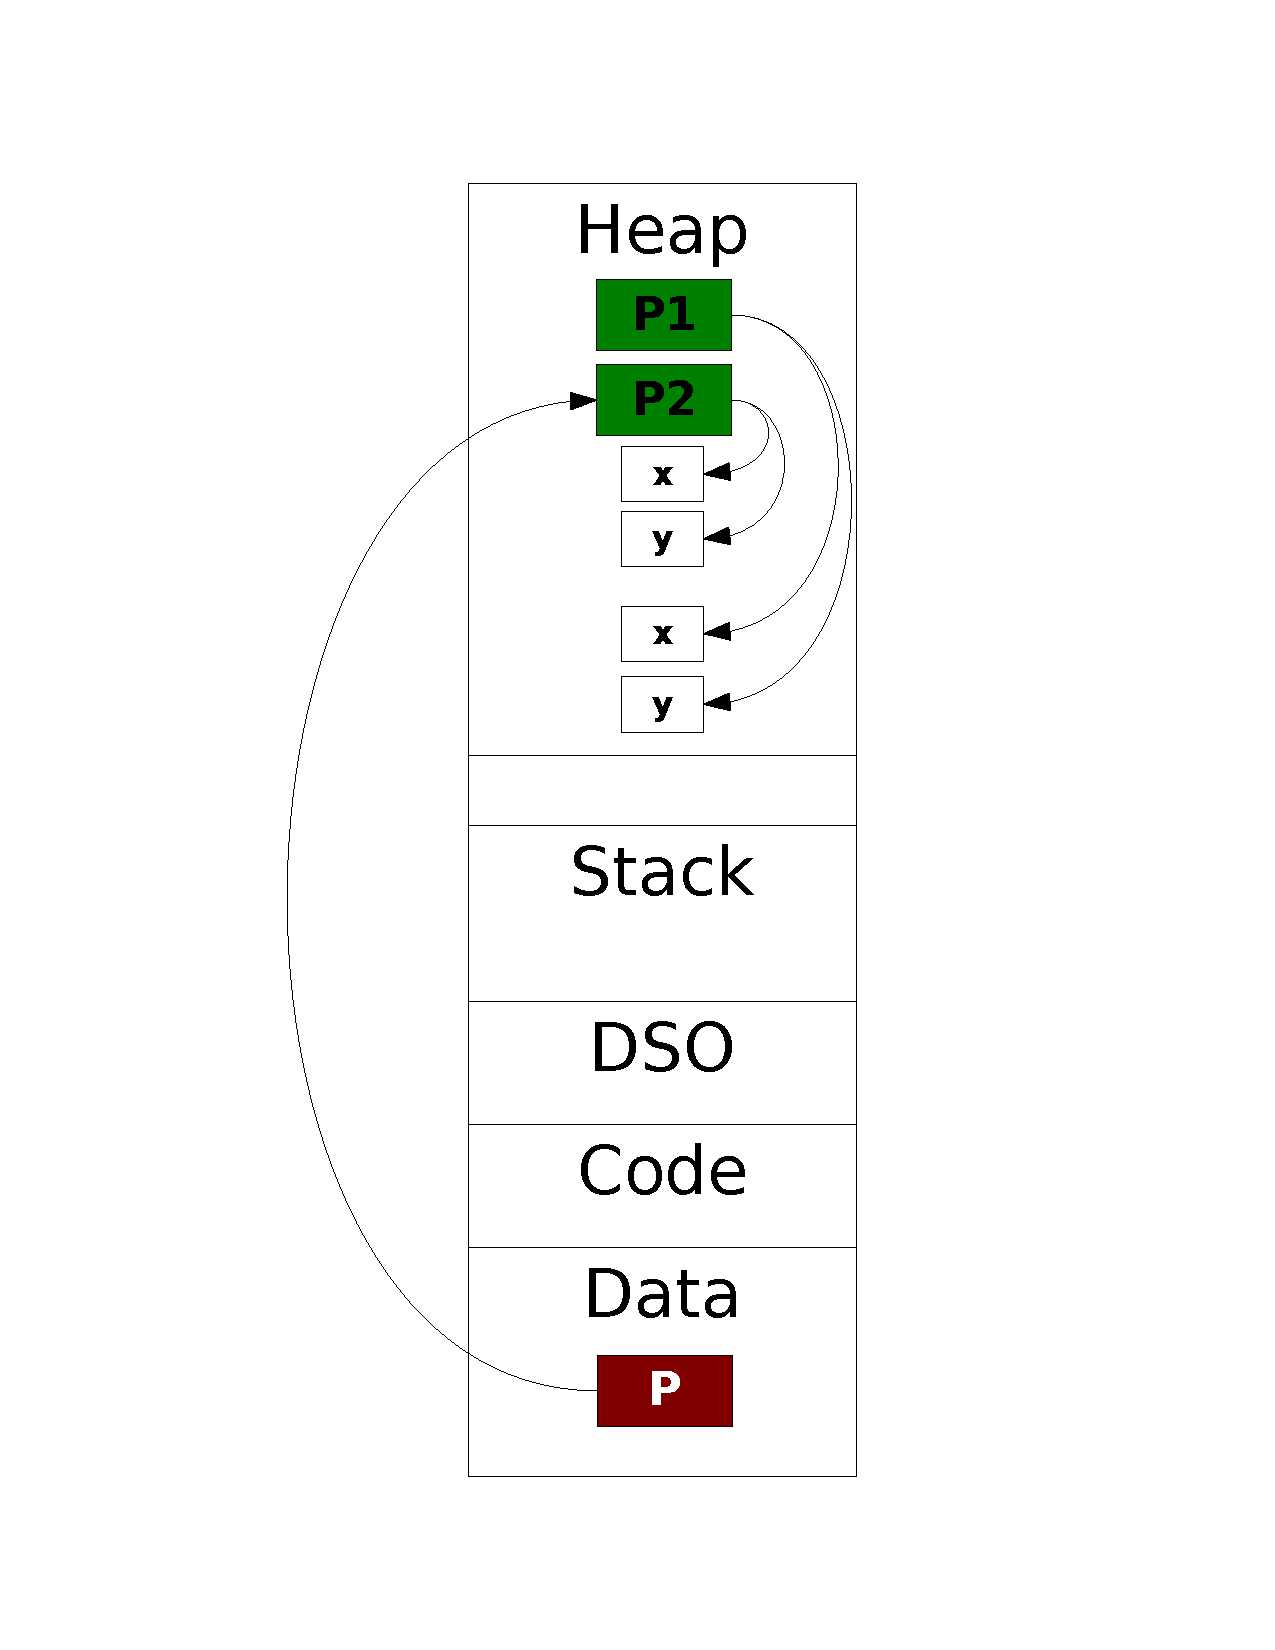
\includegraphics[width=5cm]{./Img/Memoire.pdf}
\caption{\label{fig:1}Privatisation du segment données}
\end{figure}

Enfin, il y a l'API SURF qui a pour objectif de décrire les
caractéristique de la plateforme et de la simuler. On lui fournit
donc une modèle de performance qui permettra d'estimer la durée des
calculs et des transferts.

\subsection{StarPU-MSG: Architecture générale}
\label{sec-3-2}
Comme à la base StarPU visait le modèle CPUs-GPUs, l'API la plus
proche était MSG, notamment par rapport à la création de threads et
pour la synchronisation. StarPU a donc été modifié pour pouvoir
fonctionner au dessus du simulateur SimGrid en se basant sur
MSG. Ainsi, l'application (le runtime de StarPU) est réellement
exécutée, mais les allocations mémoires des tâches ne sont pas
effectuées, les codes de calcul sont simulés et remplacés par un
délais de même pour les transferts CUDA. 

\subsection{StarPU-SMPI:Ce qui coince}
\label{sec-3-3}
Avec StarPU MPI, la modélisation est différente. On est à la fois
un environnement à mémoire partagée (entre les CPU et le GPU
d'une même machine) et un environnement à mémoire distribuée
(entre les différents noeuds). On doit donc permettre d'avoir des
modèles différents selon qu'on est entre noeud où à l'intérieur
d'un noeud. Il nous faut donc activer la privatisation de variables
entre les noeuds mais également le partage de variables à
l'intérieur de chacun noeuds. 

Pour cela nous avons besoin de faire fonctionner MSG et SMPI
ensemble. Or non seulement StarPU est essentiellement basé sur MSG
et de plus MSG et SMPI n'ont pas été prévu pour fonctionner
ensemble. Il faudra donc initialiser correctement à la fois la
partie MSG et la partie SMPI. 

Il y a un également un autre point à prendre en considération,
celui des librairies dynamiques. 

\begin{figure}[htb]
\centering
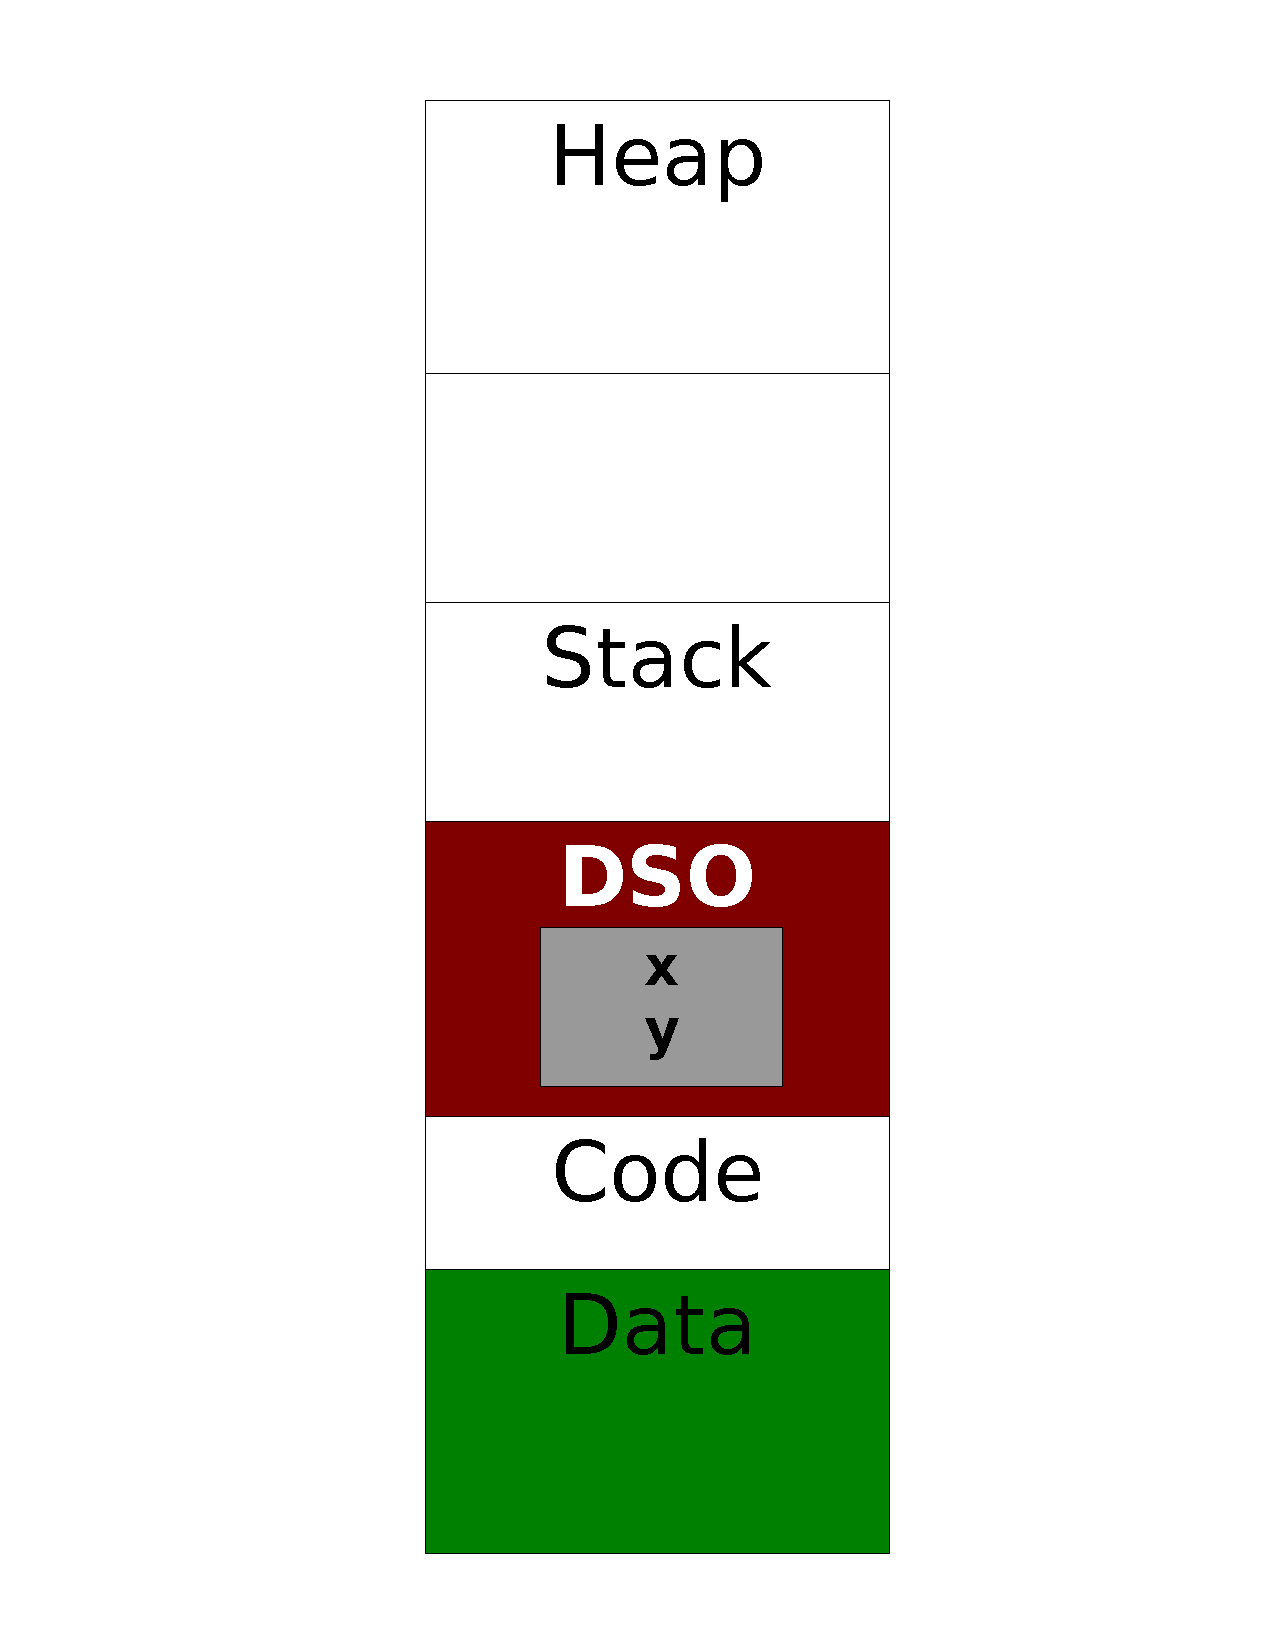
\includegraphics[width=5cm]{./Img/Dyn.pdf}
\caption{\label{fig:2}Emplacement en mémoire des bibliothèques}
\end{figure}

Dans SimGrid seul le segment données est privatisé, comme les
variables globales des librairies dynamiques ne se trouvent pas
dans ce dernier(DSO sur le schéma ci-dessus), elles restent donc
accessible accessibles à tous les processus. Nous devrons donc
également faire en sorte de privatiser les variables globales des
librairies externes entre les noeuds. 

\section{Méthodologie}
\label{sec-4}
Comme nous travaillons avec SimGrid et StarPU à la fois, nous
utilisons un dépôt complexe comprenant les deux et géré avec
l'outils submodule de \href{https://github.com/swhatelse/Journal}{git}. Ce dernier nous permet de gérer des sous
dépôt indépendemment, ainsi il est plus aisé de traiter les mises à
jours de ces derniers.

Afin de pouvoir retracer le cheminement de mon travail, mais aussi
de pouvoir garder le fil d'un jour à l'autre, un cahier de
laboratoire est tenu en org-mode et est hébergé sur github. Cela permet
également à mon tuteur de stage de savoir chaque jours l'avancement
du projet et des difficultés rencontrées.

Comme on l'a vu précédemment il est nécessaire d'apporter quelques
modifications au niveau du simulateur et de StarPU. Dans ce but, il
a été dans un premier temps nécessaire de consulter la documentation
afin de comprendre le fonctionnement et l'architecture de
SimGrid. Ensuite il a fallut explorer le code afin de déterminer où
et comment apporter les modifications. Pour cela les outils tels que
GDB et Valgrind ont été d'une aide précieuse et ont permis de
vérifier les changements de segment mémoire.

\section{Contribution}
\label{sec-5}
La toute première chose à réaliser, a été la gestion du partage du
segment de données au niveau du simulateur dans un contexte
SMPI. Comme la mémoire est partagée au sein d'un noeud, nous avons
fait en sorte que les processus d'un même noeud aient leurs segment
données en commun. Le principe est le suivant, il y a dans un
premier temps, les processus SMPI qui sont créés au lancement de
l'application avec leur propre espace de données. Puis ces derniers
peuvent à leurs tours créer de nouveau processus. Ceux-ci héritent
donc du segment de données du processus qui les a créés. SimGrid a
donc été modifié en conséquences. 

Une fois la gestion du partage mise en place, nous nous sommes
penchés sur le cas des bibliothèques dynamiques. Nous avons vu
précédemment que malgré le mécanisme de privatisation, les variables
globales présentes dans ces dernières sont partagés entre les
différents processus SimGrid. Pour contourner ce problème, nous
avons décidé d'utiliser une version statique de la bibliothèques.  

\begin{figure}[htb]
\centering
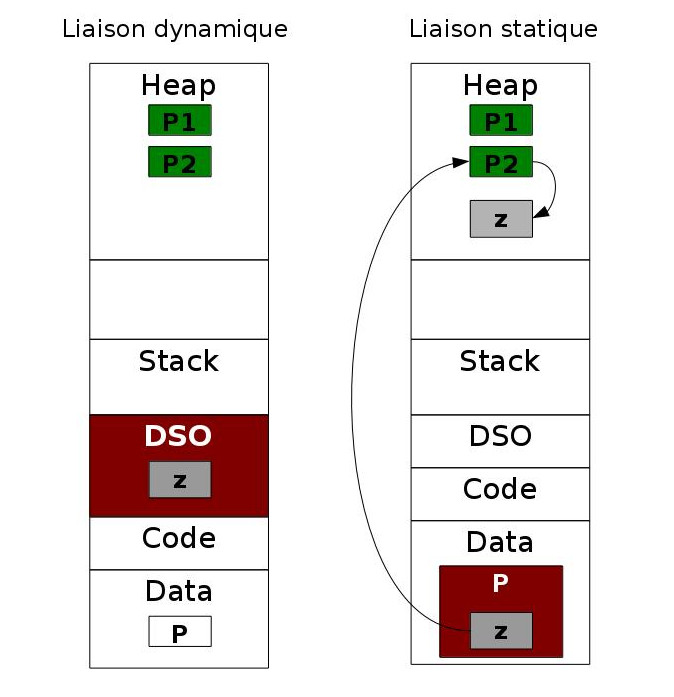
\includegraphics[width=5cm]{./Img/StaticDyn.jpg}
\caption{\label{fig:3}Emplacement en mémoire des bibliothèques}
\end{figure}

Ainsi avec une bibliothèque statique, les variables globales de
celle-ci se retrouvent dans le segment données du processus et la
gestion du partage / privatisation est géré par le mécanisme
précédent. Cependant cette solution est relativement intrusive car
elle nécessite de changer la chaîne de compilation des applications
utilisant StarPU, mais cela sera suffisants dans un premier temps. 

\section{Validation}
\label{sec-6}
\subsection{Test simple}
\label{sec-6-1}
Dans le but de tester le bon fonctionnement des modifications
apportées, un test illustrant le fonctionnement de StarPU a été
fourni et enrichi. Ce dernier permet ainsi d'isoler le problème
afin de pouvoir nous concentrer dessus. Ce test, initialise SimGrid
et la partie SMPI comme cela est fait du côté de StarPU et fait
appel à une bibliothèque dynamique et manipule des variables
globales. Ainsi lors de l'exécution de ce test, on doit pouvoir
constater que pour des processus appartenant à un même noeuds, les
valeurs des variables globales du programme et des bibliothèques
dynamiques sont bien identiques. Ce qui après plusieurs correction
a été le cas.  
\subsection{Test de StarPU - SMPI}
\label{sec-6-2}
Comme les résultats du test simples étaient ceux attendu, nous
sommes passé à un test utilisant cette fois la vrai bibliothèque
StarPU. Cette dernière est fourni avec des exemples de programme MPI
notamment d'algèbre linéaire tel que l'algorithme de Cholesky. Nous
nous sommes servi de ces dernier afin de valider les
modifications.

\section{Conclusion}
\label{sec-7}
Pour conclure, nous avons voulu voir s'il était possible de mesurer
l'influence d'un runtime dynamique sur les performances
d'applications MPI. Parmi les différentes techniques de mesures de
performances, nous avons fait le choix de la simulation / émulation
car elle nous semble la plus avantageuse, en raison de son coût, de
sa flexibilité mais aussi en terme de scalabilité.  

Pour vérifier si cette approche est effectivement possible, nous
avons modifié SimGrid afin de pouvoir faire fonctionner StarPU MPI
dessus. Nous avons donc mis en place le partage du segment données
entre les processus de même noeud et la privatisation entre les
processus de noeuds différents. 

Il reste encore de corriger le problème d'initialisation et donc les
mesures prévues n'ont pas encore pu être réalisées. Bien qu'aucune
expérimentation n'est pu être faite, les problèmes rencontrés sont
plutôt des problèmes d'ordre techniques et ne nous permettent pas
d'invalider notre hypothèse. 

Afin de pouvoir conclure sur la question, il faudra finir de
corriger la phase d'initialisation côté StarPU et également apporter
quelques correctifs à SimGrid. Ensuite nous pourrons effectuer les
simulations et les mesures. Pour ce faire les mesures seront faites
sur le logiciel Chameleon (un solveur d'algèbre linéaire basé sur
StarPU). Enfin, dans le but de valider le résultat des
expérimentations, un test grandeur nature sera fait sur Grid5000.

\section*{Acknowledgments}
Je souhaite remercier\ldots{}

\nocite{*}
\def\raggedright{}
\bibliographystyle{IEEEtran}
\bibliography{biblio}
\end{document}